% !TEX root = ./thesis.tex

\chapter*{\textbf{Appendix 3: Supplementary analysis of land use change in Monteregie \\ \hspace{1em}}}
\addcontentsline{toc}{chapter}{Appendix 3: Supplementary analysis of land use change in Monteregie}

\setcounter{chapter}{5}
\setcounter{table}{0}
\setcounter{figure}{0}

The clustering and subsequent ordination of the land use change matrices of the 177 municipalities revealed that Montérégie has 5 main profiles and land compositions (see figures \ref{fig:PCAvals}, and \ref{fig:mapvals}):
\renewcommand{\labelitemi}{$\textendash$}
\begin{itemize}[leftmargin=0.5cm]
 \item \textbf{Forest - Dominant}: have the lowest level of fragmentation and are dominated by forest.
 \item \textbf{Forest - Agriculture}: they still have a significant area of forest but fragmentation is much more pronounced.
 \item \textbf{Agriculture - Dominant}: forested habitat is scarce and most of the remaining forest is classified as “Trees” in the AAFC dataset (forest fragment of less than 1 hectare).
 \item \textbf{Urban - Medium density}: correspond to the front of the wave of urban sprawling.
 \item \textbf{Urban - High density}: urban cores make up the majority of the municipality’ area (> 50\%).
\end{itemize}

The clustering and subsequent ordination of land use change profiles showed that Montérégie has 4 different transition profiles (see figures \ref{fig:PCAtrans}, and \ref{fig:maptrans}):
\begin{itemize}[leftmargin=0.5cm]
 \item \textbf{Urban Spread / Deforestation}: forest fragmentation is progressing mainly via the growth of urban land (in the west) or development for holiday cottages (“villegiatives pressures”, in the east).
 \item \textbf{Urban Spread / Agricultural loss}: agriculture is losing ground to urban land.
 \item \textbf{Agricultural Expansion / Fragmentation}: forest is being lost to agriculture in those municipalities where forest is still quite present.
 \item \textbf{Agricultural Expansion / Deforestation}: forest is already scarce and is being replaced by agricultural land.
These results show marked regional trends with a front line of fragmentation and deforestation on both sides of the region and along the Richelieu river. \\ % (Fig. \ref{fig:map}).
\end{itemize}

%----------------------------------------------------------------------------------------------------------------

% Figures: values

% Clustering moved to appendix

% PCA
\begin{figure}[h!]
\makebox[\textwidth]{
  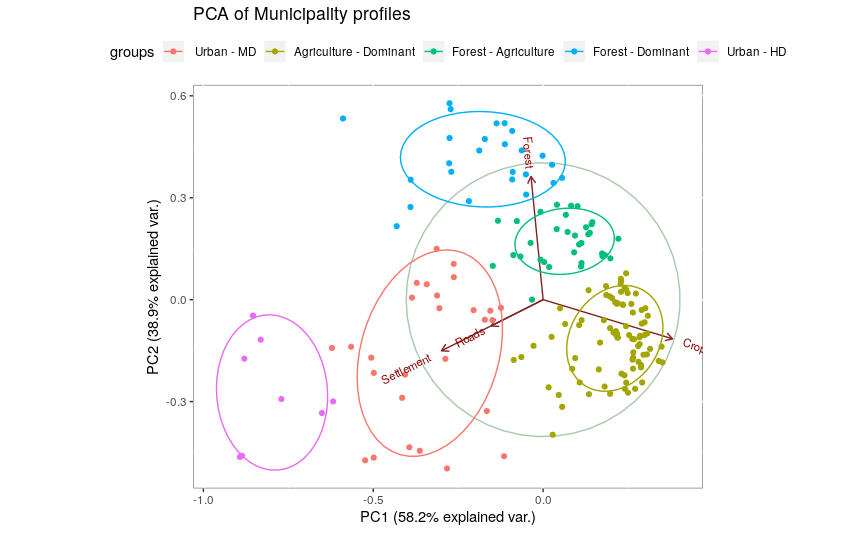
\includegraphics[width=0.8\textwidth]{thesis/figures/PCA_data_profiles.png}
}
\caption{Ordination of land use data (proportions) for municipalities.}
\label{fig:PCAvals}

% MAP
\makebox[\textwidth]{
    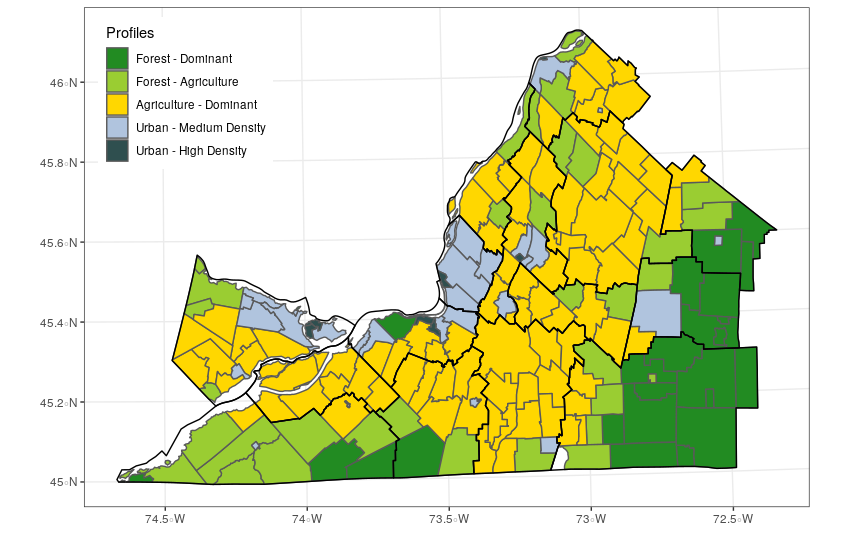
\includegraphics[width=0.8\textwidth]{thesis/figures/profiles_land_use.png}
}
\caption{Geographical distribution of the 5 profiles identified in figure \ref{fig:PCAvals}.}
\label{fig:mapvals}
\end{figure}

% Figures: Transitions

% PCA
\begin{figure}[h!]
\makebox[\textwidth]{
  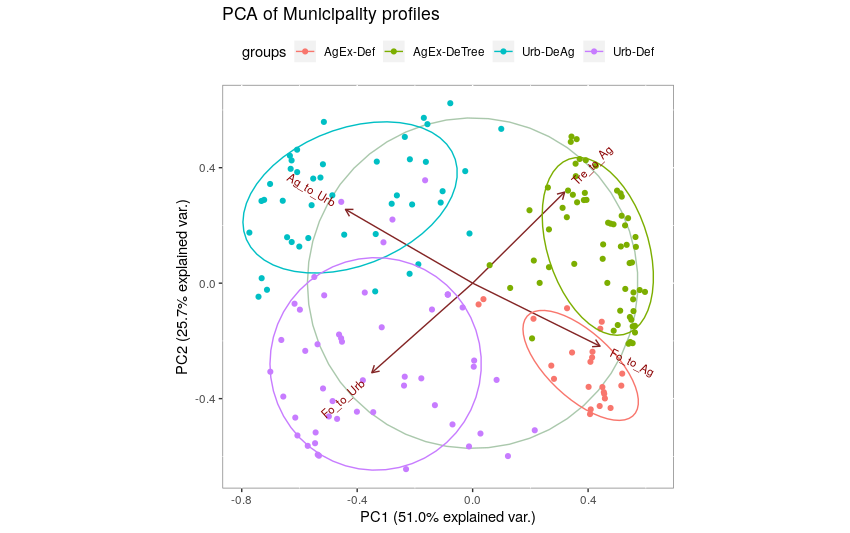
\includegraphics[width=0.8\textwidth]{thesis/figures/PCA_trans_profiles.png}
}
\caption{Ordination of land use transition data for municipalities.}
\label{fig:PCAtrans}

%MAP
\makebox[\textwidth]{
    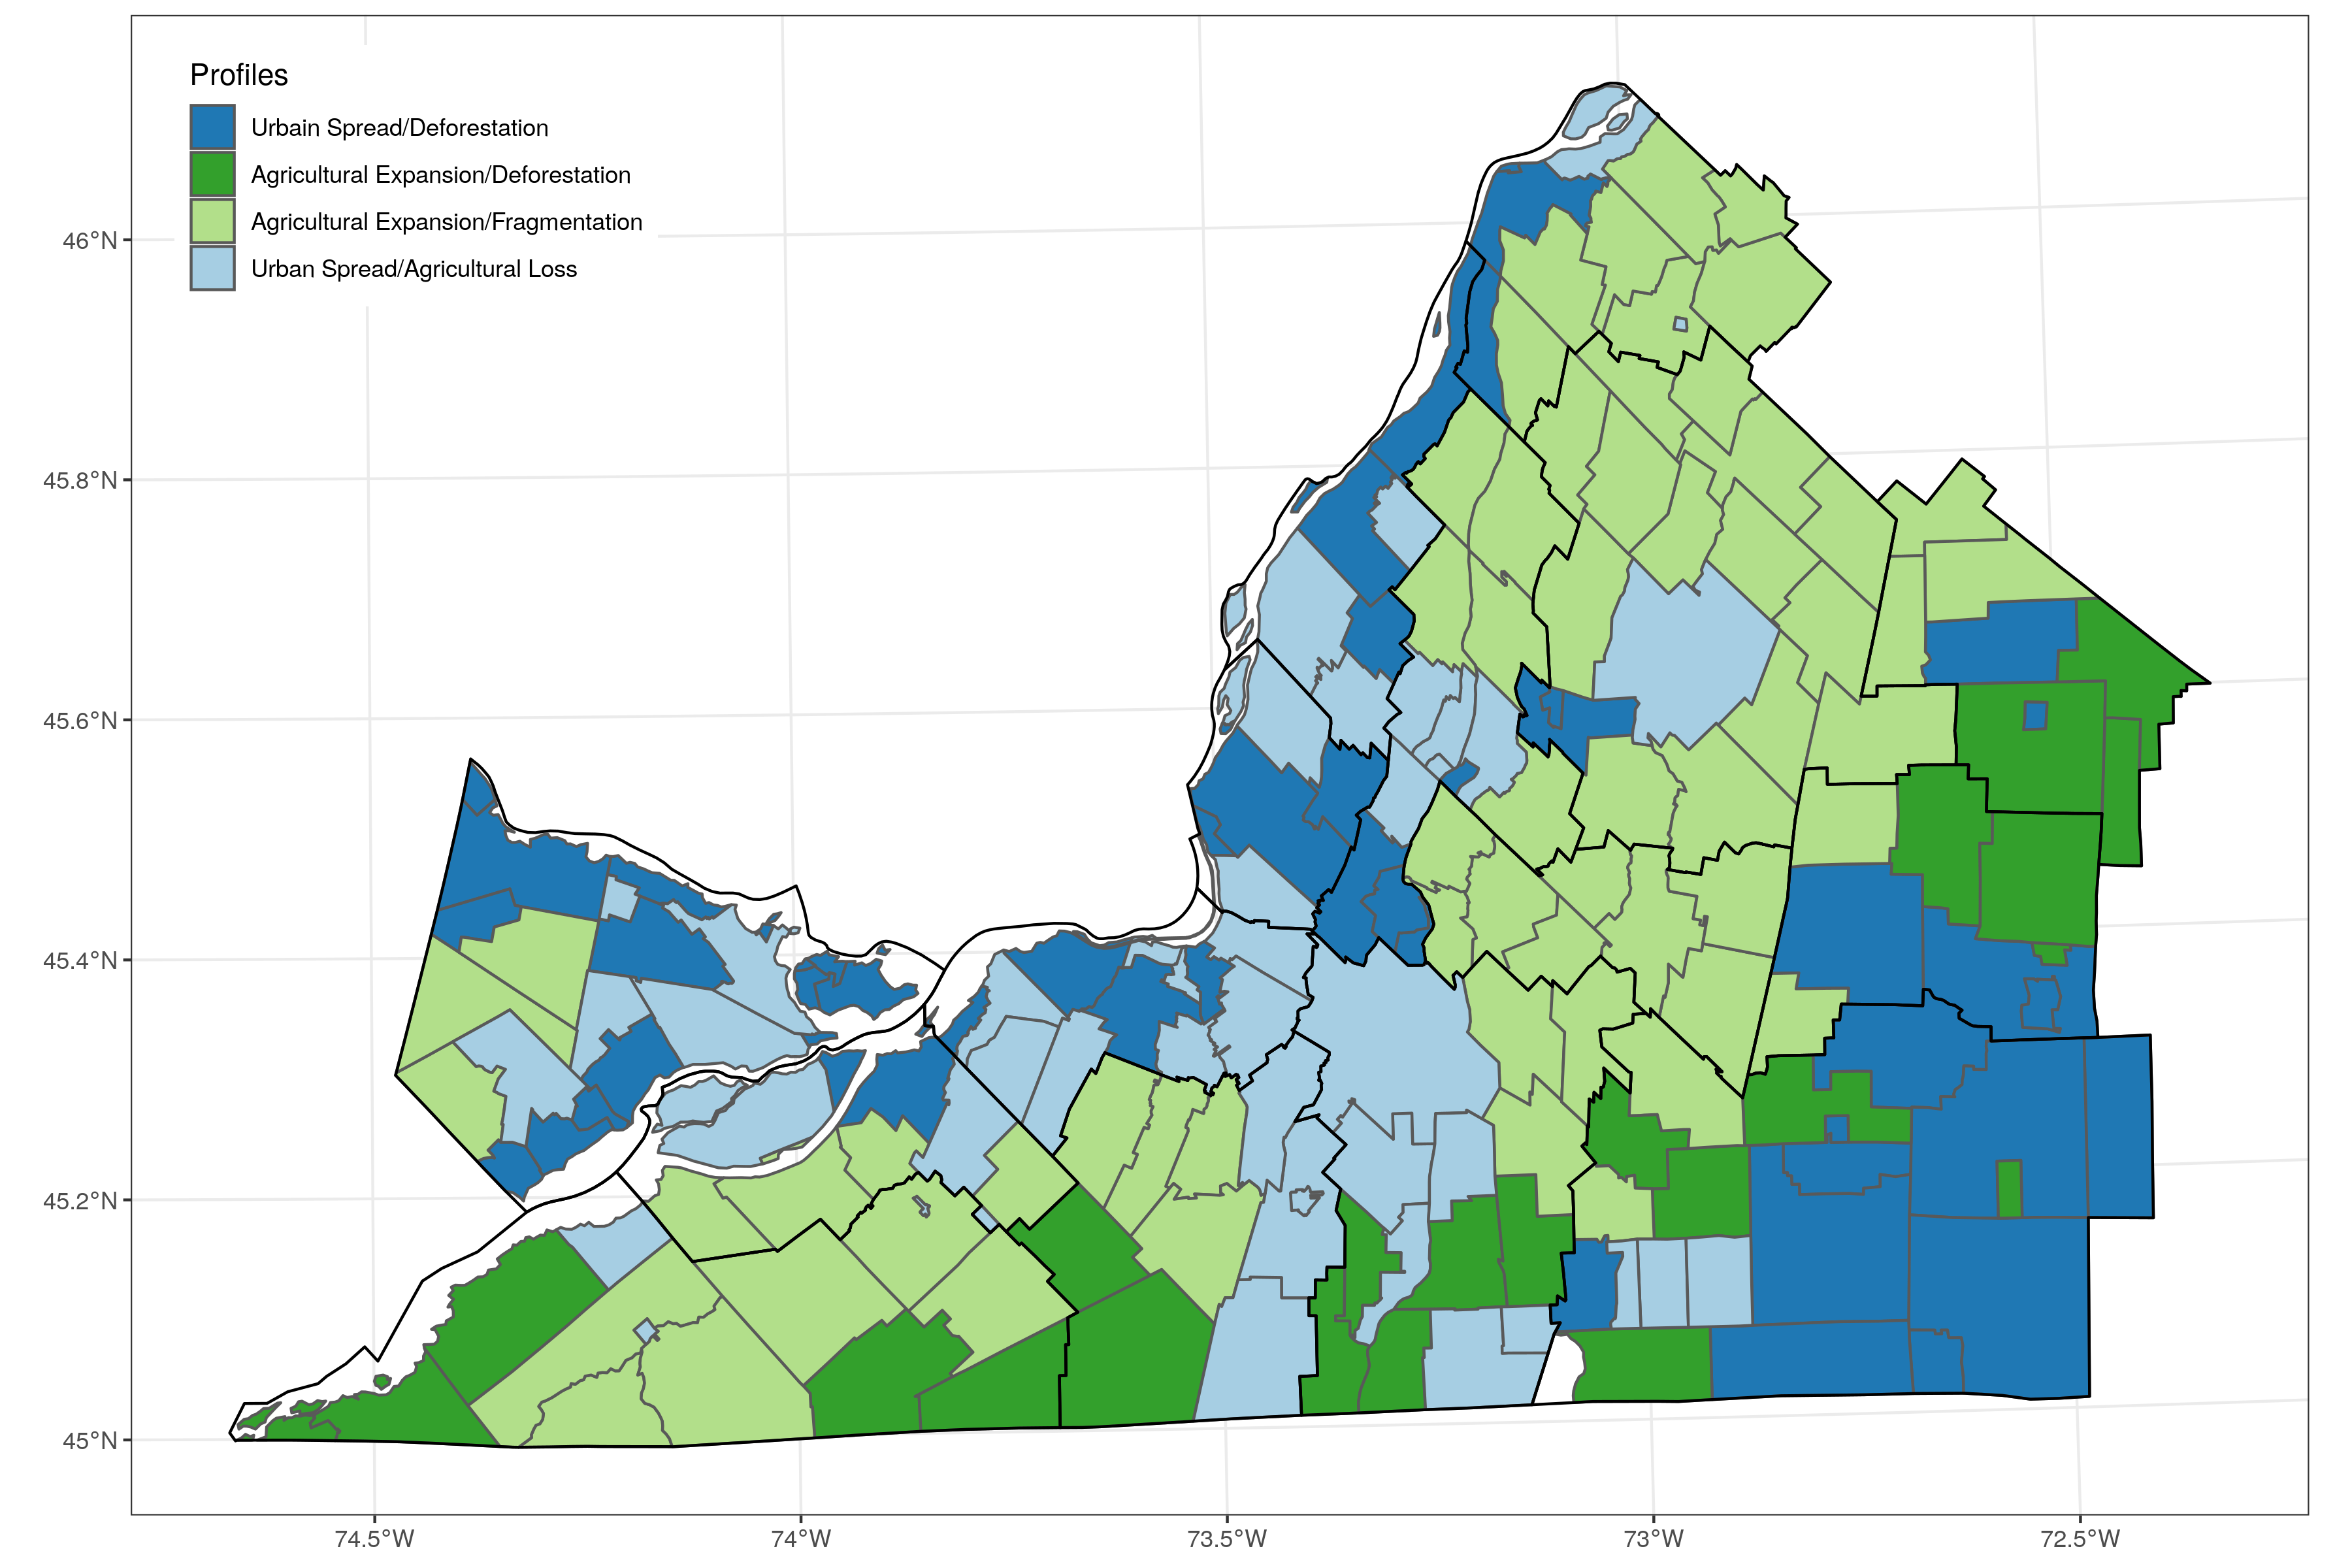
\includegraphics[width=0.8\textwidth]{thesis/figures/transition_prof_map.png}
}
\caption{Geographical distribution of the 4 change profiles identified in figure \ref{fig:PCAtrans}.}
\label{fig:maptrans}
\end{figure}

\clearpage